\chapter{Introduction}
Photonic systems provide a powerful platform for quantum information processing: photons propagate fast, have long coherence times, and can be easily manipulated \cite{Flamini2018}. Integrated photonic circuits are a particularly promising route due to their compact, on-chip designs. These have been realised experimentally with up to few hundred components, including photon pair sources and tunable phase gates \cite{Harris2017,Shadbolt2012a,Wang2018}.
However, existing technologies face the challenge of scaling up. Despite reconfigurability built into certain on-chip circuits, there is no general top-down approach to manufacturing architectures for arbitrary tasks; and state-of-the-art designs contain very few components compared to the scale needed for practical universal computing \cite{Flamini2018}. 

On the other hand, light has been used to study interference phenomena in quantum mechanical systems, where electromagnetic waves can be set up to model the interference of wavefunctions. The phenomenon we are interested in is \textit{localisation}, the confinement of waves in disordered media. Strong localisation was originally proposed by P.W.Anderson in 1958 for electrons in solids \cite{Anderson1958}, the equivalent effect has been observed using various classical waves including light, microwaves, and sound \cite{Lagendijk2009}. The key point is that disorder, i.e. randomness, gives rise to sharp spatial or spectral features which can potentially be employed for control and information processing.

This project brings together the two aspects mentioned above, and explores a new avenue for light engineering and information processing by embracing complexity. We study light transport through mesoscopic, linear waveguide networks with complex and random geometries. This brings light into the \textit{multiple scattering} regime, in contrast to the unidirectional, single scattering design in conventional architectures. Random networks present no significant design challenge in scaling up the system, and their features arising from global randomness properties are likely more robust against imperfections in manufacturing. The present report focuses on characterisation of transport and localisation effects as a function of design parameters, which paves the way for future work in using this platform for more practical engineering purposes. 

\begin{figure}[h]
  \centering
    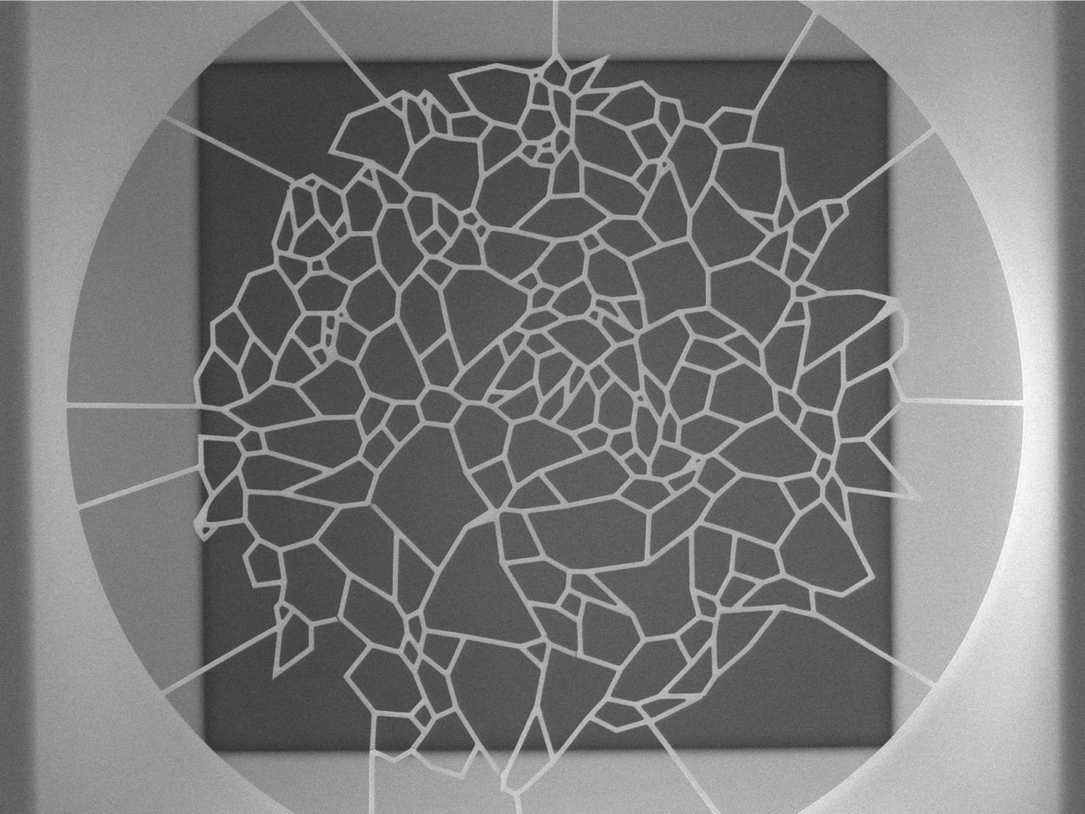
\includegraphics[width=0.55\textwidth]{ch1/fig1/network_SEM.png}
    \caption{An example complex network. Light travels along the edges of this random graph, and is allowed to back-scatter, travel in loops, and produce complex interference. The networks we study are typically tens to few-hundred microns in size.}
    \label{fig:network_SEM}
\end{figure}
We will begin by reviewing the field of linear optical quantum computing (LOQC), paying special attention to the similarity and differences between conventional architechtures and complex waveguide networks. We will also introduce in more detail the concept of multiple scattering and localisation. Chapter 2 outlines the theoretical setup we use to model complex photonic networks. Chapter 3 presents simulation results using our theoretical model, where we study both statistical and microscopic effects in such systems. Finally, chapter 4 describes the experimental setup and some preliminary measurements.

\section{Linear Optical Quantum Computing}
Linear optical quantum computing (LOQC) concerns with processing quantum information encoded in light, with optical elements such as beam splitters, phase shifters, wave plates, etc. More formally, if we expand the electromagnetic vector potential in  terms of plane wave modes
\begin{equation}
A^\mu(x,t) = \int \frac{d^3 k}{2\omega_k} \sum_{p = 1,2} \epsilon_p^\mu(k) a_p(k)e^{ikx-i\omega_k t} + \textrm{h.c.},
\end{equation}
where $\epsilon_p^\mu(k)$ are the polarization vectors and $a_p(k)$ are the corresponding annihilation operators, then a linear optics circuit has a Hamiltonian of the form
\begin{equation}
H = \sum_{jk}c_{jk}a^\dagger_ja_k,
\end{equation}
i.e. it is bilinear in the creation and annihilation operators \cite{Kok2005}.

An optical circuit essentially performs a unitary transformation on its input modes, denoted $a_j \rightarrow \sum_k U_{jk}b_j$ and $a_j^\dagger \rightarrow \sum_k U^*_{jk}b_j^\dagger$, where the overall $U$ matrix is unitary. Reck et al. \cite{Rb1994} showed that any finite discrete unitaries can be factored into $U(2)$ transformations, realisable via phase shifters and beam splitters, and can therefore be implemented by a network of linear optical elements, interfering two spatial modes at each node. This gives rise to the common architecture for LOQC chips, with unidirectional couplers between adjacent waveguide pairs. 

\subsection{Basic Elements}
In a photonic system, quantum information can be encoded in photon polarization, orbital angular momentum, propagation path, and time bin/frequency \cite{Flamini2018}.
Each of these encodings has its advantages and can be used in hybrid, but we will focus on path encoding as it is most relevant to the context of complex photonic networks.

Path encoding represents qubits (and their high-dimensional counterpart, qudits) in spatial modes. This is well suited for integrated photonic circuits, since waveguides confine photons to distinct locations on the chip. In particular, a common approach is to use a pair of waveguides to construct a ``dual-rail'' qubit: $\ket{0} = \ket 1_1 \otimes \ket 0_2$ and $\ket{1} = \ket 0_1 \otimes \ket 1_2$, where the right hand side are Fock states in the two waveguides \cite{Kok2005,Shadbolt2012a}. Efficient multi-qubit gates are achieved using the KLM scheme, which utilises gate teleportation to allow probabilistic gates to be prepared offline \cite{Knill2001}.

Integrated optical circuits are commonly manufactured using fused silica waveguides, since this material has low propagation loss and birefringence, operates in a wide range of frequencies, couples efficiently with fibers, and is robust against temperature fluctuations. These are usually realized on silicon-on-insulator, or silica-on-silicon chips. \cite{Flamini2018}.

\subsection{Quantum Random Walk}
Quantum walk is another powerful platform for quantum computation and simulation. Although different in nature from the optics-centric schemes described above, it can be implemented using photonic networks, and is capable of universal computation \cite{Childs2009}. A quantum walk generalizes the classical random walk, where at each step a ``coin state'' is ``flipped'' into some superposition in a chosen basis, and the overall state evolves conditioned on the coin state and maintains the same coherent superposition \cite{Innocenti2017}. 

Quantum walks have been implemented on bulk optics \cite{Broome2010}, fiber \cite{Defienne2016}, as well as integrated circuits \cite{Harris2017}. It can, in theory, be used to generate arbitrary high-dimensional coherent states \cite{Innocenti2017}, and under certain protocols be robust against noise in both the coin state and the environment \cite{Majury2016}. Photonic circuits have been used to simulate quantum walks of fermionic and bosonic particles \cite{Sansoni2012}, as well as transport behaviours in complex media \cite{Harris2017}.

As we shall see in the following chapters, light transport through complex networks can be viewed as a realisation of random walk on path-encoded information. Thus the universality of quantum walk provides further motivation for using complex networks as a LOQC or light state engineering platform.

\section{Multiple scattering in disordered media}
Although first proposed for solid state systems, multiple scattering and localisation are wave phenomena that can take place in any disordered medium. \textit{Disorder} refers to the degree of randomness present in a physical system; for instance in Anderson's original paper it refers to randomness in single-cite potential energies in a lattice \cite{Anderson1958}. 

Multiple scattering occurs when waves travel through a disordered medium and produces complex interference patterns \cite{Ott2012}. This phenomenon was first experimentally investigated in semiconductor powder \cite{Wiersma1997} and colloidal suspensions \cite{Lawandy1994}. Sending quantum states of light (squeezed states) into a multiple scattering medium has been shown to produce quantum correlations between output spatial modes \cite{Smolka2009,Smolka2012}. These results suggest light engineering potential in our complex networks, which produce multiple scattering in lower dimensions, and a more controlled manner. A disordered medium can be characterised as a linear-response medium, where multiple scattering is modelled using the scattering matrix and random matrix theory \cite{Rotter2017}, and is shown to be able to mix various input quantum states \cite{Ott2010}. We shall see in the following chapters the parallels between this theoretical approach and our model. Finally, wavefront shaping combined with multiple scattering have been used to focus classical light through turbid media \cite{Katz2011}, which inspires us to employ input wavefront shaping to explore the full range of transport features in complex photonic networks. 

Localisation is the spatial confinement of waves in disordered media arising from multiple scattering. The physics is complex and not fully understood, but an intuitive picture for the physical principle is illustrated in Fig.\ref{fig:multiple_scattering}: a wave propagates from point A to point B and then back along two paths in opposite directions, which interfere constructively and increase the probability of remaining at A. However, this is unlikely to happen under a certain disorder threshold, whence the probability of propagating from A to B can be added incoherently (i.e. in squares) instead of interfered coherently, resulting in \textit{diffusion}. The presence of enhanced back-scattering is referred to as \textit{weak localisation}, while the regime where the wave is brought to a complete halt is termed \textit{strong}, or \textit{Anderson localisation}. \cite{Lagendijk2009}

\begin{figure}[h]
  \centering
    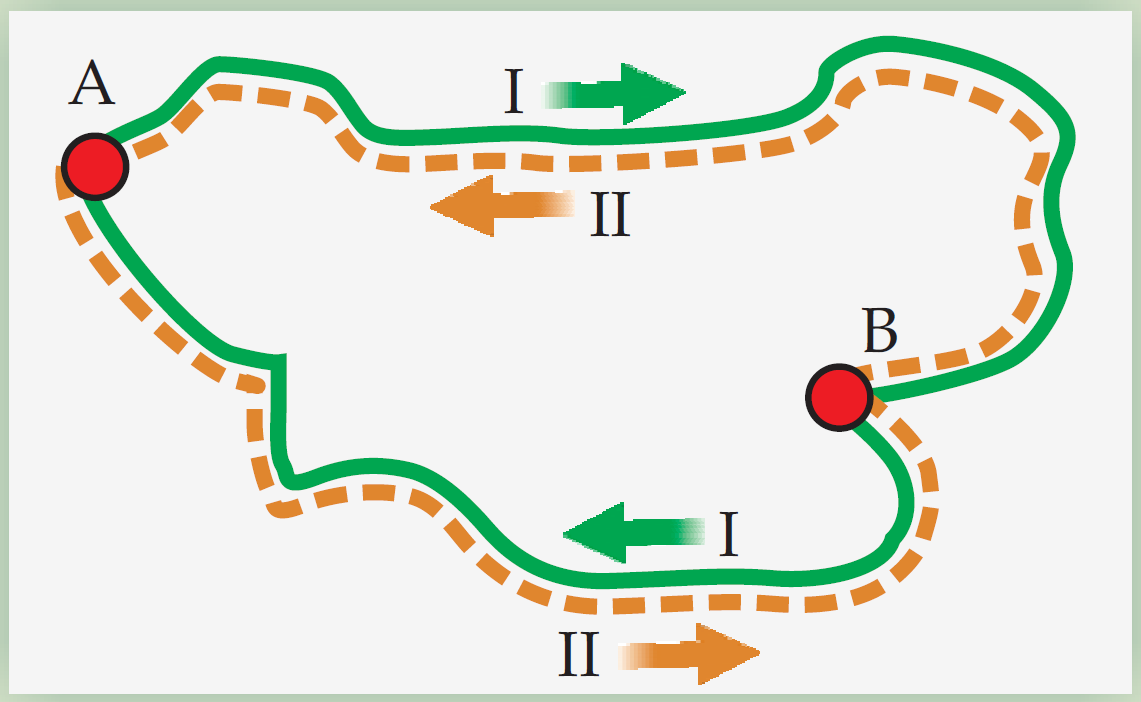
\includegraphics[width=0.6\textwidth]{ch1/fig1/multiple_scattering}
    \caption{Illustration of how multiple scattering can lead to localisation: paths I and II interfere constructively, increasing the probability of remaining at A. \cite{Lagendijk2009}}
    \label{fig:multiple_scattering}
\end{figure}

It might seem counter-intuitive to study transport behaviours in a localised system. However, localisation does not necessarily lead to low transmission. In 1994 J.Pendry showed that in 1D systems localised modes can be strung together into conducting ``necklace states'' \cite{Pendry1994}, which has been observed experimentally in optical systems \cite{Bertolotti2005}.

Having motivated the investigation of multiple scattering and transport of light through complex nanophotonic networks, we will now move on to study this system in detail.



% \section{Complex photonic networks}
% Nanoscale complex photonic networks, as used in this project, are meshes of subwavelength waveguides, in which light propagate along the edges and scatter at the nodes. For quantum light states, such a system can be treated as a quantum graph \cite{Kuchment2004}. In the classical regime, light traveling through such a network can be modeled by Maxwell's equations on a graph, as described in \cite{Gaio2017}:

% Along an edge traveling from node $i$ to node $j$ with length $L_{ij}$, a propagating mode simply picks up a complex phase factor $k$: $E(x_j) = E(x_j)e^{ikL_{ij}}$. The wave equations along the edges are constrained by boundary conditions at the nodes. In particular, we require that (a) $E^r(x_i) = E^s(x_j)$ for edges $r$ and $s$ meeting at node $i$, and (b) $\sum_r\frac{dE(x)}{dx}\big|_{x=x_i} = 0$ for all edges meeting at node $i$, with the positive direction of $x$ being all in-going or out-going. These conditions are equivalent to enforcing Laplace's equation; a graph Laplacian is defined as $\nabla^2 = A-D$, where $A$ is the adjacency matrix of the graph and $D$ the connectivity degree matrix.

% The network approach has several advantages as a quantum computation and simulation framework. First of all, it can be scaled up to increase the level of complexity without much difficulty in terms of fabrication: the networks we are working with can contain several hundred nodes \cite{Gaio2017}, at least an order of magnitude more than the number of interaction sites in a integrated circuit fabricated via a top-down design process \cite{Harris2017}. On the other hand, a planer geometry and minimal out-of-plane scattering losses \cite{Gaio2017} confines the system to two dimensions, which provides richer dynamics than 1D systems \cite{Bertolotti2005}, while remaining more computationally tractable than 3D systems \cite{Wiersma1997}.


% \subsection{Multiple Scattering in Disordered Media}
% One reason why complex photonic networks have potential computing and simulation power is that these nanoscale systems are in the multiple scattering regime \cite{Gaio2017}; on the other hand, under the coupled-dipole approximation \cite{Yurkin2007}, multiple scattering of waves can be described as discrete scattering elements with propagation paths connecting them, fitting a network/graph description. 

% Multiple scattering occurs when waves (or photons or states, in the quantum case) travel through a disordered medium and produces complex interference patterns \cite{Ott2012}. This phenomenon was first investigated in semiconductor powder \cite{Wiersma1997} and colloidal suspensions \cite{Lawandy1994}. Sending quantum states of light (squeezed states) into a multiple scattering medium has been shown to produce quantum correlations between output spatial modes \cite{Smolka2009,Smolka2012}. The disordered medium can be characterized as a linear-response medium, where multiple scattering is modeled using the scattering matrix and random matrix theory, and is shown to be able to mix various input quantum states \cite{Ott2010}. Light scattering through a disordered medium is therefore similar to a complex linear optical circuit, or a random quantum walk. Since our photonic networks produce multiple scattering of light, this comparison illuminates the potential of photonic networks as a quantum state engineering platform.


% \subsection{Fabrication}
% Photonic networks similar to those used in this project can be fabricated by electro-spinning polymethyl methacrylate (PMMA) nanofibers (doped with Rhodamine-6G) onto TEM grids. These result in waveguides with diameter of $200-500 nm$, and on average $26.5\mu m$ in length between overlaps/nodes. The nodes are bonded via annealing in a nitrogen atmosphere.\cite{Gaio2017} This process forms a random network, characterized by node degrees and link/edge lengths. Similar devices have been tested for plasmonic systems, where light scattered from gold hyperuniform disordered surfaces showed reciprocal space engineering features \cite{Castro-Lopez2017}. Networks used in this project will be designed random networks fabricated using an etching process: this will provide us better handle on the statistical qualities of the network, and further reduce out-of-plane loses at nodes.

% Networks fabricated using nanofibers can be interfaced with a single photon source using a technique described in \cite{Gaio2016}: similar PMMA nanofibers can be electro-spun onto TEM plates, with CdSeTe quantum dots embedded in the fibers. These devices improve upon evanescently coupled fibers, do not require nanolithography to fabricate, can operate with a broadband response at room temperature, and achieve broadband coupling of up to 31\% of emitted light \cite{Gaio2016}. 


% \subsection{Detection and Characterization}
% This project will investigate both classical (supercontinuum) light transport and quantum (entangled two-photon) state multiple scattering across the network, bearing in mind the goal of quantum state engineering and synthesis. The output states of the network need to be accessed and characterized, which will be done using correlations and speckle patterns.

% Optical speckle is the interference of scattered light, for example through a disordered medium. They contain distributions--functions of intensity that provide information about the light state. For one photon, one could look at properties such as the speckle contrast ($\mathcal{V} = \langle I^2\rangle/\langle I\rangle^2 - 1$); for two photons, the speckle pattern can be used to extract information such as the Schmidt number.\cite{Beenakker2009}

% The first part of the project will focus on classical light transport: light will be injected into the network via grating couplers, and the output will be characterized using spectrometers coupled to one or more outgoing edges. \cite{Fryett2018}.






